%%%%%%%%%%%%%%%%%%%%%%%%%
%% Header for standard beamer presentation
%%
%%  PresentationHeader.tex
%%
%%%%%%%%%%%%%%%%%%%%%%%%%

\documentclass[english,10pt]{beamer}

%%%%%%%%%%%%%%%%%%%%
%% Include general header where common packages are defined
%%%%%%%%%%%%%%%%%%%%

% general packages without options
\usepackage{amsmath,amssymb,bbm}




%%%%%%%%%%%%%%%%%%%%
%% Idem general commands
%%%%%%%%%%%%%%%%%%%%

%%% Commands

\newcommand{\noun}[1]{\textsc{#1}}


%% Math

% Operators
\DeclareMathOperator{\Cov}{Cov}
\DeclareMathOperator{\Var}{Var}
\DeclareMathOperator{\E}{\mathbb{E}}
\DeclareMathOperator{\Proba}{\mathbb{P}}

\newcommand{\Covb}[2]{\ensuremath{\Cov\!\left[#1,#2\right]}}
\newcommand{\Eb}[1]{\ensuremath{\E\!\left[#1\right]}}
\newcommand{\Pb}[1]{\ensuremath{\Proba\!\left[#1\right]}}
\newcommand{\Varb}[1]{\ensuremath{\Var\!\left[#1\right]}}

% norm
\newcommand{\norm}[1]{\| #1 \|}


% amsthm environments
\newtheorem{definition}{Definition}



%% graphics

% renew graphics command for relative path providment only ?
%\renewcommand{\includegraphics[]{}}






\usetheme{Warsaw}

\setbeamertemplate{footline}[text line]{}
\setbeamercolor{structure}{fg=purple!50!blue, bg=purple!50!blue}

\setbeamercovered{transparent}


% shortened command for a justified frame
\newcommand{\jframe}[2]{\frame{\frametitle{#1}\justify{#2}}}



%%%%%%%%%%%%%%%%%%%%%
%% Begin doc
%%%%%%%%%%%%%%%%%%%%%

\begin{document}



\title{Thesis Progress Meeting}


\author{J.~Raimbault$^{1,2}$}

\institute{$^{1}$G{\'e}ographie-cit{\'e}s (UMR 8504 CNRS)\\
$^{2}$LVMT (UMR-T 9403 IFSTTAR)}


\date{October 23th 2015
}


%%%%%%%%%%%%%%%%%%%%%%%%%%%%%%%%
\begin{frame}
\titlepage
\end{frame}

%\begin{frame}
%\tableofcontents
%\end{frame}
%%%%%%%%%%%%%%%%%%%%%%%%%%%%%%%%


%\section{Projects Organization}

%\jframe{Projects Organization}{
%   \includegraphics[width=\textwidth,height=0.8\textheight]{figures/orgaProjects}
%}



\section{Achieved Work}


\jframe{Achieved Work (by projects)}{
\begin{itemize}
\item Incompressible Tasks :
\begin{itemize}
\item Biblio/Reading Records [1w]
\item Conference (ECQTG)/Seminars [1,5w]
\item Meetings/Organisation [1,4w]
\end{itemize}
\item Cybergeo Project [1,4w]
\item Synthetic Data/Density Model [1,5w]
\item Algorithmic Systematic Review (incl. technical tools) [1w]
\item Lutecia Model [2w]
\item Space Matters [1w]
\item Thematic Paper/Plan construction [0.4w]
\item Monitorat [2,8w]
\end{itemize}

\bigskip

$\rightarrow$ 1M (25\%) ``lost'' in incompressible tasks ; 0.75M (20\%) in Monitorat.

}



\section{Thesis Plan}


\jframe{Proposition of a Thesis plan}{
 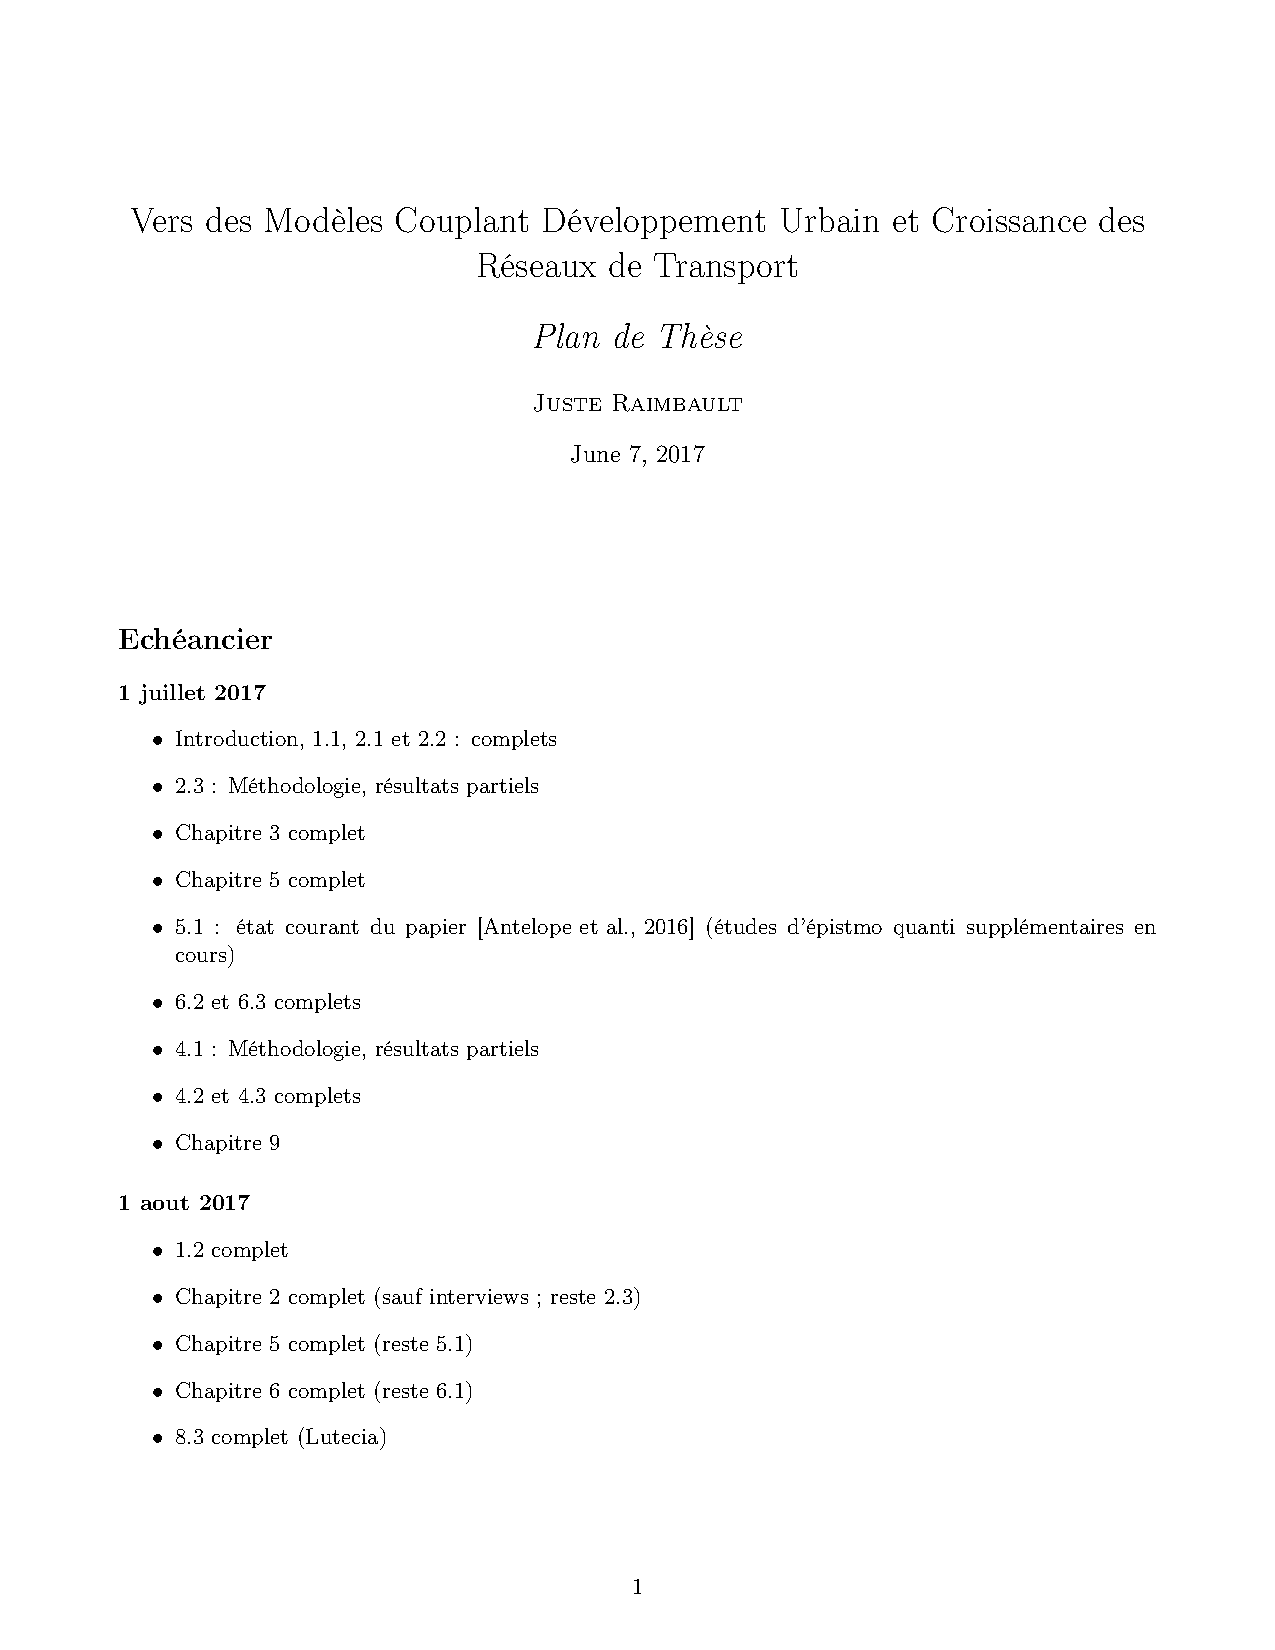
\includegraphics[angle=90,height=\textheight]{plan}
}






%%%%%%%%%%%%%%%%%%%%%%%%%%%%%%%%
\jframe{Next steps (until November 23th)}{
\begin{itemize}
\item \emph{Survive} cumulation Monitorat/Research
\item Density Model : grid computation, write paper - ETA 1w
\item Lutecia : Validation procedure and paper - ETA 1w
\item Cybergeo : advanced results - ETA 1w
\item Finish Thematic Paper - ETA 0.5w
\item Network-Density Stats and correlated Synthetic Data - ETA 0.5w
\end{itemize}
}






%%%%%%%%%%%%%%%%%%%%%%%%%%%%%%%%
%\begin{frame}[allowframebreaks]
%\frametitle{References}
%\bibliographystyle{apalike}
%\bibliography{/Users/Juste/Documents/ComplexSystems/CityNetwork/Biblio/Bibtex/CityNetwork}
%\end{frame}
%%%%%%%%%%%%%%%%%%%%%%%%%%%%%%%%


\end{document}
